\documentclass[a4paper,14pt]{extreport}

\usepackage[T1,T2A]{fontenc}
\usepackage[utf8]{inputenc}

\usepackage{style/bsumain}
\usepackage{style/bsudiplomatitle14}
\usepackage{blindtext}
\usepackage{float}

\subfaculty{Кафедра биомедицинской информатики}
\title{Изучение методов описания химических соединений для примемения в алгоритмах машинного обучения}
\author{Малыщик Аким Андреевич}
\mentor{Тузиков Александр Васильевич \\
        профессор кафедры БМИ}
\reviewer{Орлович Юрий Леонидович \\
          заведующий каведры БМИ}

\usepackage{graphicx}
\begin{document}
\maketitle
\setcounter{page}{2}
\begin{center}
  \large\bfseries{РЕФЕРАТ}
\end{center}

Курсовой проект, 20 стр., 5 иллюстр., 6 источников.

\textbf{Ключевые слова:} ДЕСКРИПТОРЫ, МОЛЕКУЛЯРНЫЕ ФИНГЕРПРИНТЫ, SMILES.

\textbf{Объекты исследования -} дескрипторы химических соединений, алгоритмы машинного обучения на основе дескрипторов.

\textbf{Цель исследования --} изучение существующих молекулярных дескрипторов и алгоритмов на их основе.

\textbf{Методы исследования --} системный подход, изучение соответствующей литературы и электронных источников.

\textbf{В результате исследования} исследованы графовые структуры, молекулярные фингерпринты и SMILES, изучены алгоритмы обработки дескрипторов, рассмотрены архитектуры нейросетей на основе SMILES-описаний.

\textbf{Области применения --} хемоинформатика, медицина, фармацевтика.

\newpage
  {
    \renewcommand{\contentsname}{Содержание}
    
    \tableofcontents
  }

  \chapter*{Введение}
  \addcontentsline{toc}{chapter}{Введение}
  \label{c:introduction}
  В последнее время нашу планету наводнили вирусы, угрожающие всему населению земного шара. Вот уже два года пандемия коронавируса SARS-Cov2 не даёт спокойно жить людям. Естественно, лучшие умы планеты делают всё возможное, чтобы найти лекарство. Однако, на полный цикл от нахождения нужного соединения до появления вакцины на полках аптек нужны годы, которых, вообще говоря, нет. Таким образом, приходится отказываться от традиционных методов создания лекарств и исследовать, на каком этапе процесс можно ускорить, полагаясь на современные технологии. В частности, последнее десятилетие ознаменовалось прорывом в области искусственного интеллекта. На данный момент методы и алгоритмы машинного обучения начинают использоваться практически повсеместно, поэтому возникает естественная идея применить их и в сфере разработки вакцин, а именно — на стадии генерации новых соединений.
  
Понятное дело, что последние несколько столетий химики не сидели сложа руки и успели открыть огромное множество химических соединений. Для их хранения существуют базы данных вроде PubChem, в которых приведены подробные сведения обо всём. Из них можно выбирать соединения, обладающие определёнными свойствами, синтезировать или покупать готовые, и проверять их эффективность в борьбе с вирусами.
Однако, мир не так тесен, как иногда кажется, и соединения, которые есть в базах — лишь верхушка айсберга. Гораздо большее число веществ до сих пор не исследовано и не получено в принципе, а среди таких веществ ведь могут быть и потенциально полезные в данной задаче. Как уже было отмечено, для получения новых соединений можно использовать генеративные нейросети. На данный момент наиболее перспективными архитектурами для генерации веществ являются рекуррентные нейросети, автокодировщики, а также генеративно-состязательные сети. Они будут рассмотрены далее.

В общем виде все нейросети работают схожим образом: на вход модели подаётся вектор каких-то данных, которые пропускаются через слои с нейронами, и на выходе получается какой-то ответ (в нашем случае, хотелось бы получить сгенерированное соединение). Основная сложность и проблема в том, что не существует универсального способа закодировать любое вещество, отразив все его свойства, который был бы лучше всех остальных в любой задаче. Таким образом, задачи данного курсового проекта:

\begin{enumerate}
\item Изучить существующие на данный момент дескрипторы химических соединений
\item Исследовать их преимущества и недостатки
\item Рассмотреть алгоритмы генерации веществ на основе существующих дескрипторов
\end{enumerate}

В дальнейшем работу над проектом можно будет продолжить, проведя сравнительный анализ дескрипторов для какой-нибудь конкретной мишени, и сделать выводы касательно наиболее удачного способа описания веществ в конкретной ситуации.

Существует множество способов описать вещество. В рамках данного проекта абсолютно все рассмотрены не будут, предпочтение будет отдано тем методам, которые потенциально перспективны для использования в области машинного обучения.
Итак, основные способы представить химическое соединение в памяти компьютера:
\begin{enumerate}
  \item Графы структур соединений
  \item Бинарные векторы свойств (молекулярные фингерпринты)
  \item Линейные представления: SMILES, IChI, SLN
\end{enumerate}

В данном проекте рассматривается каждый из способов по отдельности, изучаются преимущества и недостатки каждого, а также исследуются области применения рассматриваемых методов.

  
  
  
  

  
  
  \chapter{Графы структур}
  \label{c:graphs}
  
  С точки зрения математики, графом $G(V,E)$ называется совокупность непустого множества $V$ и множества $E$ неупорядоченных пар различных элементов множества $V$. Множество $V$ называется ''множеством вершин'', множество $E$ называется ''множеством рёбер''.

$$G(V,E) = \left \langle V,E \right \rangle, \quad  V  \ne \varnothing , \quad E \subseteq V \times V , \quad  \left \{ v,v \right \} \notin E, \quad v \in V .$$
  
  Поскольку молекулы состоят из атомов и связей между ними, идея представить химическое соединение в виде графа его структуры кажется вполне естественной. Существует несколько способов представления графов в памяти компьютера:
  \begin{enumerate}
	\item Матрица смежности
	\item Матрица расстояний
	\item Матрица инцидентности
	\item Матрица связей
\end{enumerate}
Рассмотрим каждый из них.
  
  

  \section{Матрица смежности}
  \label{s:matrix_1_sec}
  При таком способе хранения соединения заводится матрица размера N*N, где N — число атомов в соединении. Матрица заполняется нулями, если связь между атомами отсутствует и единицами, если связь есть. Поскольку матрица смежности симметрична, расход памяти, занимаемой матрицой, можно уменьшить, если хранить только её треугольную форму. Также для большей эффективности представления и экономии памяти из матрицы можно исключить связи с атомами водорода, ведь их можно будет при необходимости восстановить по правилам валентности. Недостатком матрицы смежности является то, что в ней не содержится информации о типах связей между атомами в молекуле. Таким образом, информация, которую содержит такая матрица, позволяет построить граф молекулы, однако по ней невозможно восстановить полную структуру соединения.
  \section{Матрица расстояний}
  \label{s:matrix_2_sec}
  Матрица расстояний, как и матрица смежности, симметрична, и её размер (NxN) также зависит только от числа атомов в соединении. Матрица содержит расстояния между соответствующими атомами в молекуле. К матрице расстояний применимы те же оптимизации по расходу памяти, что и к матрице смежности.
  
  Расстояния между атомами можно задавать двумя способами. Первый - с помощью евклидовой метрики:
  $$d(a,b)=\sqrt{(a_1-b_1)^2+(a_2-b_2)^2+(a_3-b_3)^2}.$$
  В таком случае расстояния выражаются в ангстремах или нанометрах. Второй способ - топологическое расстояние (минимальное количество связей в графе соединения между атомами A и B). 
  
  Таким образом, матрицы расстояний имеют те же проблемы, что и матрицы смежности: информации в них недостаточно для полного восстановления структуры соединения. Однако, они позволяют воссоздать расположение атомов в трёхмерном пространстве.


  \section{Матрица инцидентности}
  \label{s:matrix_3_sec}
  Матрица инцидентности, в отличие от остальных матриц, представляет собой прямоугольную матрицу MxN, её размеры зависят от числа атомов и числа связей в молекуле. Как и матрица смежности, матрица инцидентности показывает лишь наличие либо отсутствие какой-либо связи, без указания её типа. Размеры матрицы инцидентности можно уменьшить, если не рассматривать атомы водорода.

  \section{Матрица связей}
  \label{s:matrix_4_sec}
  Матрица связей решает проблему всех рассмотренных выше матриц. Как и матрица смежности, она представляет собой квадратную матрицу NxN. Но эта матрица не является бинарной, она хранит порядки связей между атомами, а не только нули и единицы. Порядок связи для несвязанных между собой атомов формально полагается равным 0. Соответственно, двойная связь обозначается числом 2, тройная - числом 3, и т.д.

К матрице связей можно применить те же методы сокращения расхода памяти, что и к матрице смежности (удаление атомов водорода, симметричной части). Данная матрица содержит достаточно информации для полного восстановления структуры соединения. Однако, в случае наличия в соединении ароматических связей, для которых нет конкретного значения порядка связи, представление молекулы с помощью данной матрицы будет неоднозначным, и необходимы дополнительные соглашения касательно того, как обозначать такие связи.
\begin{figure}[htp]
\centering
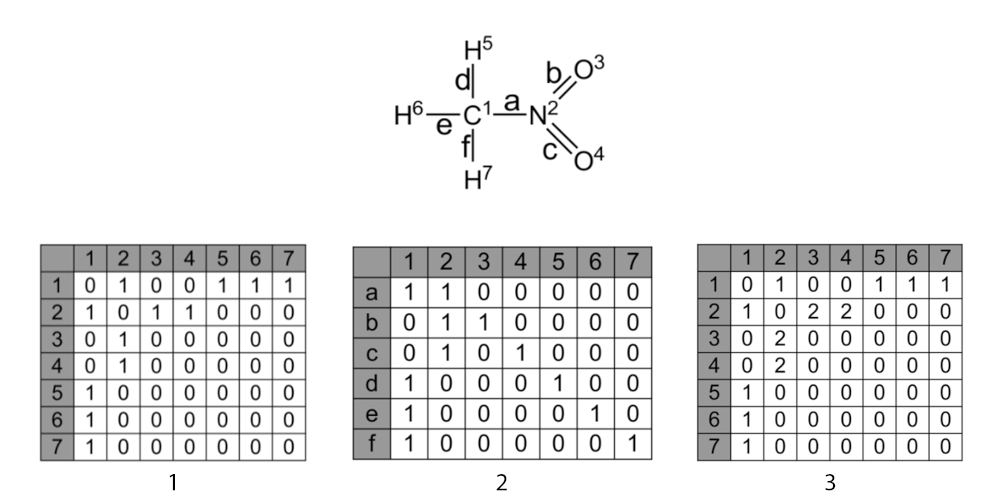
\includegraphics[scale=0.35]{images/нитрометан.png}
\caption{Представление молекулы нитрометана \\матрицей смежности (1), матрицей инцидентности (2), матрицей связей (3)}
\label{nitromethane}
\end{figure}

  \section{Применение графов соединений в машинном обучении}
  \label{s:graphs_applications}
Графовые структуры данных могут быть полезными для предварительной обработки данных о соединениях, закодированных другими способами. К примеру, особенностью SMILES-описаний химических соединений является их неуникальность. Чтобы избежать проблемы дублирования соединений и ускорить молекулярный докинг, все сгенерированные нейросетью SMILES-соединения можно канонизировать, после чего удалить явные дубликаты. Алгоритм канонизации SMILES-описаний основан на алгоритме канонизации графа, то есть для его работы необходимо преобразовать соединение из SMILES в какое-нибудь из матричных представлений, произвести процедуру канонизации помеченного графа, и выполнить обратное преобразование в SMILES.

Тем не менее, разрабатывать нейронные сети на основе графовых структур смысла не имеет. Во-первых, большинство матричных структур не позволяет хранить достаточно информации о свойствах соединения, а значит, нейросеть не сможет выявить закономерности, необходимые для генерации соединений с аналогичными свойствами. Во-вторых, из матричного представления не всегда возможно однозначно восстановить закодированное соединение, что делает мало полезным генерацию веществ в таком виде и заставляет задуматься о применении других способов описания молекул.


  \chapter{Молекулярные фингерпринты}
  \label{c:fingerprints}
  Молекулярные фингерпринты – достаточно известный способ векторизации молекулярных данных, он часто используется при обучении с учителем, а также для поиска соединений со схожими свойствами.
  
Молекулярные фингерпринты — это битовые строки, в которых каждый бит отвечает за наличие или отсутствия какого-либо фрагмента в соединении. При этом не существует универсальных меток для каждого бита. Молекулярный фингерпринт, как правило, генерируется из самой молекулы. 

  \section{Алгоритм генерации фингерпринтов}
  \label{s:fp_generation_sec}
  Алгоритов генерации молекулярных опечатков существует несколько. Рассмотрим алгоритм, используемый компанией Daylight. Этот алгоритм исследует молекулу и генерирует признаки для следующих паттернов (подструктур):
  \begin{itemize}
	\item паттерн для каждого атома
	\item паттерн, представляющий каждый атом и его ближайших соседей (а также связи между ними)
	\item паттерн, представляющий каждую группу атомов, соединённых путями длиной до 2 связей
	\item паттерн, представляющий каждую группу атомов, соединённых путями длиной до 3 связей
	\item и т.д.
  \end{itemize}
К примеру, для молекулы $\bold{OC=CN}$ алгоритм бы сгенерировал следующие паттерны:


\begin{center}
\begin{tabular}{cccc}
	Длина пути 0: & C & O & N\\
	Длина пути 1: & OC & C=C & CN\\
	Длина пути 2: & OC=C & C=CN\\
	Длина пути 3: & OC=CN
\end{tabular}
\end{center}


Список полученных паттернов исчерпывающий: таблица содержит все подструктуры исходной молекулы. Очевидно, на практике количество паттернов, необходимых для описания больших соединений может быть просто огромным. При этом, чтобы производить какие-либо операции над фингерпринтами, требуется фиксированная длина отпечатка для всех молекул в датасете. Но тогда, если использовать вектор слишком большой длины для маленьких соединений, большая часть вектора будет заполнена нулями. И наоборот, при использовании слишком маленьких фингерпринтов для больших соединений весь фингерпринт будет заполнен единицами (и, возможно, будет при этом хранить не всю информацию о соединении). Чтобы избавиться от этих проблем, фингерпринты подвергают процедуре фолдинга.


  \section{Фолдинг фингерпринтов}
  \label{s:fp_folding_sec}
 Процесс фолдинга начинается с фиксированного размера фингерпринта, достаточно большого для полного представления структуры молекулы. Далее фингерпринт сворачивается (англ. fold): происходит его разделение на две части, которые складываются при помощи логического оператора OR. На выходе получается более короткий фингерпринт с более высокой плотностью информации на бит. Процесс фолдинга можно повторить несколько раз, пока не будет достигнута желаемая плотность информации.
 
Однако, таким образом может быть потеряна часть информации. Рассмотрим фингерпринты подструктуры P и молекулы M. Если все биты подструктуры P изначально находятся в молекуле M, то это будет справедливо и после фолдинга. С другой стороны, если хотя бы один бит из P изначально не в M, то после фолдинга может оказаться, что подструктура P содержится в M. Это может привести к тому, что при виртуальном скрининге найдётся больше соединений с подструктурой P, чем нужно. С каждой процедурой фолдинга будет увеличиваться вероятность найти ''лишние'' молекулы, однако фингерпринт будет занимать в два раза меньше пространства.

Таким образом, генерировать фингерпринты фиксированной длины необязательно, достаточно сгенерировать фингерпринт любой длины, представляющий полную структуру соединения, и с помощью фолдинга привести его к необходимому фиксированному размеру. 
 
  
  \section{Сравнение фингерпринтов}
  \label{s:fp_comparing_sec}
Для сравнения двух молекулярных отпечатков соединений достаточно сравнить их побитово. Рассмотрим фингерпринты A и B. При их сравнении возможны 4 ситуации, представленные в таблице 2.1.
  
\begin{table}  
\begin{center}
\begin{tabular}{|c|c|c|c|}
\hline
	& 0 & 1 & Сумма\\
\hline
	0 & d & b & b + d\\
\hline
	1 & a & c & a + c\\
\hline
	Сумма & a + d& b + c & n\\
\hline
\end{tabular}
\caption{Побитовое сравнение фингерпринтов A и B}
\end{center}
где:
\begin{itemize}
\item a – количество битов, равных единице в фингерпринте А и нулю в B.

\item b – количество битов, равных единице в фингерпринте B и нулю в A.

\item c – количество битов, равных единице в обоих фингерпринтах.

\item d – количество битов, равных нулю в обоих фингерпринтах.
\end{itemize}
\end{table}

\begin{table}[H]
На основе данных показателей существует множество метрик для сравнения двух соединений. Некоторые из них представлены в таблице 2.2.
\begin{center}
\begin{tabular}{|c|c|c|}
\hline
	Метрика & Область значений & Формула\\[2ex]
\hline
	Дайс & $[0, 1]$ & $\frac{2c}{(a+c)+(b+c)}$\\[5ex]
\hline
	Евклид & $[0, 1]$ & $\sqrt{\frac{c + d}{a + b + c + d}}$\\[5ex]
\hline
	Манхэттен & $[1, 0]$ & $\frac{a + b}{a + b + c + d}$\\[5ex]
\hline
	Танимото & $[0, 1]$ & $\frac{c}{a + b + c}$\\[5ex]
\hline
	Симпсон & $[0, 1]$ & $\frac{c}{min((a+c),(b+c))}$\\[5ex]
\hline
\end{tabular}
\caption{Метрики для сравнения фингерпринтов}
\end{center}
\end{table}
\newpage
\begin{lstlisting}[language=Python, caption=Использование метрики Дайса и библиотеки RDKit для сравнения двух фингерпринтов Моргана]
>>> from rdkit.Chem import MolFromSmiles
>>> from rdkit.Chem.AllChem import GetMorganFingerprint
>>> from rdkit.DataStructs import DiceSimilarity
>>> molecule_1 = MolFromSmiles('Cc1ccccc1')
>>> molecule_2 = MolFromSmiles('Cc1ncccc1')
>>> fingerpint_1 = GetMorganFingerprint(molecule_1, 2)
>>> fingerpint_2 = GetMorganFingerprint(molecule_2, 2)
>>> DiceSimilarity(fingerpint_1,fingerpint_2)
0.55...
\end{lstlisting}


  \section{Распространённые виды фингерпринтов}
  \label{s:fp_types_sec}

  \subsection{Фингерпринты Моргана}
  \label{ss:fp_morgan_subsec}
  Моргановские фингерпринты – это 2048-битные векторы, названные в честь ученого, который предложил алгоритм их генерации. Алгоритм Моргана генерации молекулярных фингерпринтов работает следующим образом:
Для каждого атома в соединении вычисляются следующие показатели:
\begin{enumerate}
\item количество ближайших соседей (кроме атомов водорода)
\item количество связей у атома (без учета связей с атомами водорода)
\item атомный номер
\item атомная масса
\item количество связей с атомами водорода
\item принадлежит атом циклу (1) или нет (0)?
\end{enumerate}
Данные показатели хэшируются. Таким образом у каждого атома появляется его идентификатор (хэш-значение). Первая итерация завершена. 

Далее для каждого атома заводится массив его соседей и связей между ними, отсортированный по хэш-значениям атомов. Этот массив также хэшируется, а полученное значение становится новым идентификатором атома. Таким образом, на первой итерации алгоритма произойдёт хэширование отдельных атомов, на второй – хэширование атомов с их соседями диаметра 1, на третьей – с соседями диаметра 2 и т.д. После завершения итерационного процесса производят конкатенацию хэш-значений всех атомов, и с помощью фолдинга полученный вектор переводят в бинарный вектор длины 2048 бит.

  \subsection{Структурные ключи MACCS}
  \label{ss:fp_maccs_subsec}
  Структурные ключи отличаются от обычных фингерпринтов тем, что в них заранее определено, за что отвечает каждый бит. Ключи MACCS (Molecular ACCess System), также известные как ключи MDL, названы так в честь разработавшей их компании. Существует две разновидности ключей MACCS (одна содержит 960 ключей, другая – её подмножество из 166 ключей). Краткое описание каждого из ключей можно найти в репозитории компании.

  \subsection{Другие виды фингерпринтов}
  \label{ss:fp_other_subsec}
  Помимо двух вышеописанных, существуют, например, фингерпринты PubChem (длины 881 бит, применяются для поиска по одноименной базе данных). Также иногда имеет смысл заменить хэш-функции в алгоритме создания фингерпринта на дифференцируемые функции, что позволит “обучать” фингерпринт вместе с нейросетью, оптимизируя таким образом фингерпринт под конкретную задачу и достигая больших успехов, чем при работе со стандартными фингерпринтами.
  
  \section{Применение фингерпринтов в машинном обучении}
  \label{s:fp_application}
  Молекулярные фингерпринты получили широкое применение в машинном обучении. На их основе создают модели для предсказания токсичности молекул, растворимости веществ, и прочих показателей, расчет которых экспериментальным путем потребовал бы гораздо больших финансовых затрат.
  
Тем не менее, молекулярные фингерпринты имеют один большой недостаток: обычно, когда у вас есть фингерпринт, не существует простого метода восстановления изначальной структуры соединения, которое представлено в виде фингерпринта. Это оказывается особенно важным при работе с соединениями, которые сгенерированы с помощью искусственного интеллекта, и которые при этом необязательно могут быть найдены в базах данных существующих молекул.
Поэтому на данных момент при работе с искусственным интеллектом чаще используются SMILES описания, точнее SMILES-вектора.

  
  \chapter{SMILES}
  \label{c:smiles}
  SMILES (Simplified Molecular Input Line Entry System) - линейная нотация для ввода и представления молекул и реакций. SMILES содержит ту же информацию, что и расширенные матрицы связей. Основная причина, по которой SMILES полезнее матрицы связей, в том, что SMILES скорее языковая структура, чем структура данных. При этом алфавит и количество правил SMILES-кодирования невелико, что позволяет, во-первых, легко кодировать и декодировать соединения вручную, а во-вторых, позволяет без проблем применять к SMILES те же методы машинного обучения, что и к естественным языкам.
Еще одним преимуществом языка SMILES является компактность записи соединений с его помощью (относительно других линейных нотаций и прочих методов описания соединений).

\begin{table}[H]
\begin{center}
\begin{tabular}{|l|l|l|l|}
\hline
	Формула & Код SMILES & Код InChI\\
\hline
	$CH_3CH_2OH$ & CCO & InChI=1S/C2H60/c1-2-3/h3H,2H2,1H3\\
\hline
	$CH_3CH=O$ & CC=O & InChI=1S/C2H4O/c1-2-3/h2H,1H3\\
\hline
	$CH_3COOH$ & CC(O)=O & InChI=1S/C2H4O2/c1-2(3)4/h1H3,(H,3,4)\\
\hline
\end{tabular}
\caption{Сравнение представлений SMILES и InChI}
\end{center}
\end{table}


Из таблицы видно, что для кодирования с помощью SMILES, как правило, требуется в разы меньше символов, чем для кодирования с помощью международного химического идентификатора InChI. Также соединения в виде SMILES занимают в памяти компьютера на 50-70\% меньше пространства, чем те же соединения, представленные в виде матриц связей их атомов.

  \section{Правила кодирования SMILES}
  \label{s:smiles_coding_sec}
  SMILES нотация представляет собой не разделенную пробелами последовательность символов. Запись SMILES получается в результате обхода в глубину вершин молекулярного графа.
Как правило, SMILES не включает в себя атомы водорода (связи C-H, N-H, O-H, S-H), поскольку их можно восстановить по правилам валентности.
\newpage
\begin{table}[H]
\begin{center}
\begin{tabular}{|c|c|c|}
\hline
	C & метан & $CH_4$\\
\hline
	P & фосфин & $PH_3$\\
\hline
	N & аммиак & $NH_3$\\
\hline
	S & сероводород & $H_2S$\\
\hline
	O & вода & $H_2O$\\
\hline
	Cl & соляная кислота & $HCl$\\
\hline
\end{tabular}
\caption{Примеры молекул без атомов водорода в SMILES}
\end{center}
\end{table}

Циклы в графах соединений разъединяются, места разъединения обозначаются числами, показывающими наличие связей в исходной структуре соединения.

\begin{figure}[htp]
\centering
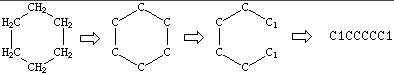
\includegraphics[scale=1.20]{images/Screenshot from 2021-12-04 16-34-09.png}
\caption{Разъединение циклов в SMILES}
\label{cycles}
\end{figure}

Точки ветвления обозначаются круглыми скобками.

\begin{figure}[htp]
\centering
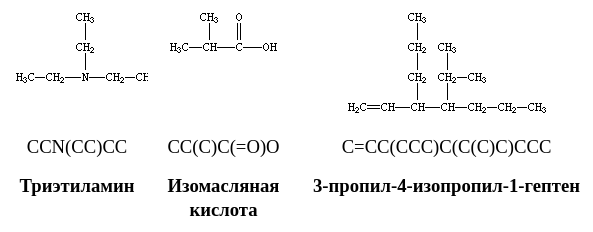
\includegraphics[scale=0.80]{images/Screenshot from 2021-12-04 16-45-58.png}
\caption{Примеры соединений с точками ветвления}
\label{branches}
\end{figure}

Двойную связь обозначают символом =, тройную – символом \#.

\begin{table}[H]
\begin{center}
\begin{tabular}{|l|c|c|}
\hline
	C=O & Формальдегид & $CH_2O$\\
\hline
	C=C & Этен & $CH_2=CH_2$\\
\hline
	O=C=O & Углекислый газ & $CO_2$\\
\hline
	C\#N & Цианид & $HCN$\\
\hline
\end{tabular}
\caption{Примеры соединений с двойными и тройными связями}
\end{center}
\end{table}

Для обозначения конфигурации асимметрического тетраэдрического атома углерода используются символы @ (против часовой стрелки) и @@ (по часовой стрелке). Для обозначения конфигурации следует смотреть на хиральный центр со стороны заместителя, стоящего в строке SMILES перед этим центром. В полном соответствии с последовательностью в строке SMILES трёх других заместителей определяется часовое направление, которое указывается как @ или @@ возле асимметрического атома углерода, заключаемого в квадратные скобки.

Атом водорода в конфигурационных кодах указывается обязательно и, если помещается в строке SMILES сразу после хирального центра, то может вместе с ним заключаться в квадратные скобки.


\begin{figure}[htp]
\centering
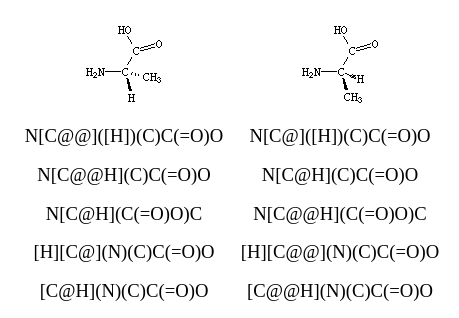
\includegraphics[scale=0.80]{images/Screenshot from 2021-12-04 16-57-53.png}
\caption{Разные конфигурации одних и тех же структур}
\label{configs}
\end{figure}

Символами $/\ \backslash$ обозначается конфигурация относительно двойной связи.

\begin{figure}[htp]
\centering
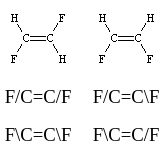
\includegraphics[scale=1.00]{images/Screenshot from 2021-12-04 16-59-41.png}
\caption{Примеры кодирования цис- и транс- изомеров}
\label{isomeric}
\end{figure}




\begin{table}[H]
Изотопы обозначаются числами перед атомами.
\begin{center}
\begin{tabular}{|c|c|}
\hline
	Код SMILES &  Название\\
\hline
	[12C] & Углерод-12\\
\hline
	[13C] & Углерод-13\\
\hline
	[13CH4] & С-13 метан\\
\hline
\end{tabular}
\caption{Примеры кодирования изомеров в SMILES}
\end{center}
\end{table}




\begin{table}[H]
Ионизация обозначается символами + и - с указанием числа ионов, если оно не равно единице.
\begin{center}
\begin{tabular}{|l|l|}
\hline
	[H+] & протон\\
\hline
	[Fe++2] & катион железа (II)\\
\hline
	[OH-] & гидроксильный анион\\
\hline
	[Fe++] & катион железа (II)\\
\hline
	[NH4+] & катион аммония\\
\hline
\end{tabular}
\caption{Примеры кодирования катионов и анионов в SMILES}
\end{center}
\end{table}

  \section{Применение SMILES в машинном обучении}
  \label{s:smiles_application}
  Как уже было отмечено, использование представления химических соединений с помощью языка SMILES позволяет применять к соединениям те же подходы, что и, например, при работе с текстами. Это значит, что для генерации соединений подойдут те же архитектуры нейронных сетей, что и для генерации текстов. На данный момент написано множество генераторов соединений, основанных на рекуррентных нейронных сетях (точнее, на архитектуре LSTM), а также на автоэнкодерах и гетероэнкодерах.
  \subsection{Предварительная обработка SMILES-датасета}
  \label{ss:smiles_preprocessing_subsec}
  В ходе проведённых исследований было выяснено, что из входных данных имеет смысл исключать следующие соединения:
  \begin{enumerate}
  \item Не валидные SMILES-представления
  \item Соединения без атомов углерода
  \item Соединения с атомами, не входящими в состав потенциальных лекарств (отличными от H, C, N, O, P, S, F, Cl, Br, I)
  \item Соединения длиной более 120 символов
  \item Соединения с молекулярной массой > 1000 а.е.м.

  \end{enumerate}
  
    После фильтрации имеет смысл избавиться от дубликатов по названиям соединений, а также по SMILES (можно удалить как явные дубликаты, так и сравнить канонические SMILES-представления и удалить совпадающие).
    
   Далее закодированные в SMILES соединения с помощью one-hot кодирования переводят в бинарные вектора размера (максимальная длина SMILES)x(количество уникальных символов в SMILES), после чего датасет можно использовать для обучения моделей нейронных сетей.
  
  \subsection{Архитектуры нейросетей на основе SMILES}
  \label{ss:fp_other_subsec}
  Ещё одним преимуществом SMILES по сравнению с фингерпринтами является то, что SMILES представления последовательны. В отличие от фингерпринтов, которые содержат информацию об отдельных фрагментах структуры молекулы, SMILES описания позволяют анализировать всю структуру целиком, а не отдельные фрагменты. Последовательность SMILES делает возможным использовать данные представления в рекуррентных нейронных сетях в целом и в LSTM-сетях в частности. LSTM-слои позволяют генерировать следующие символы формулы в SMILES на основе предыдущих, причём в контексте всей структуры, а не только нескольких последних символов. 
  
  Другой перспективной архитектурой для генерации SMILES-описаний являются автокодировщики (англ. autoencoders). Данная архитектура позволяет генерировать соединения, сжимая их и добавляя шум к сжатым данным (кодирование), а после восстанавливая соединения (декодирование). Для реализации кодировщиков можно применять LSTM-слои. Архитектуру можно использовать как для обучения без учителя, так и для semi-supervised learning (к примеру, в latent space автокодировщика можно добавить нейрон с желаемой энергей связи, что позволит получить на выходе соединения с заданным свойством).
  
  Дальнейшей идеей развития архитектуры автоэнкодеров являются гетероэнкодеры. Данная архитектура представляет собой несколько кодировщиков и несколько декодировщиков, что позволяет, во-первых, оптимизировать вычисления (можно использовать кодировщики и декодировщики базового уровня), а, во-вторых, получать на выходе соединения разных типов (каждый декодировщик будет генерировать соединения своим особым образом). К примеру, можно воспользоваться неуникальностью SMILES представлений, и в качестве входных данных в разные кодировщики подать все возможные SMILES-представления одного и того же соединения. Тогда на выходе из разных декодировщиков можно будет получить разные представления одного и того же соединения (при идеальных кодировщике и декодировщике), либо несколько соединений с похожей структурой и свойствами.
  
  Помимо гетероэнкодеров, существует множество архитектур, являющихся, по сути, улучшениями автоэнкодеров...
  
  Таким образом, многие архитектуры нейронных сетей, подходящие для работы с естественными языками, нашли своё применение и в сфере генерации потенциальных лекарственных соединений.
  

  \chapter*{Заключение}
  \addcontentsline{toc}{chapter}{Заключение}
  \label{c:conclusion}
 В ходе проекта была собрана теоретическая база для дальнейших исследований. А именно:
  \begin{enumerate}
  \item Исследованы такие методы описания химических соединений, как графы, фингерпринты и SMILES
  \item Изучены алгоритмы для работы с данными методами (канонизация, фолдинг и др.)
  \item Рассмотрены архитектуры нейронных сетей, в которых применимы данные методы
  \item Изучены варианты предварительной обработки SMILES-датасета
  \item Изучена библиотека RDKit.
  \end{enumerate}
  

  \chapter*{Список использованной литературы}
  \addcontentsline{toc}{chapter}{Список использованной литературы}
  \label{c:literature}


\end{document}
